%%%%%%%%%%%%%%%%%%%%%%%%%%%%%%%%%%%%%%%%%%%%%%%%%%%%%%%%%%%%%%%%%%%%%%%%%%%
% % Plantilla para un artculo en LaTeX en espaol.  %
%%%%%%%%%%%%%%%%%%%%%%%%%%%%%%%%%%%%%%%%%%%%%%%%%%%%%%%%%%%%%%%%%%%%%%%%%%%

\documentclass[12pt,twoside,onecolumn]{article}

% Esto es para poder escribir acentos directamente:
%\usepackage[latin1]{inputenc}
\usepackage[utf8]{inputenc}
\usepackage{makeidx} \usepackage{multirow} \usepackage{titlesec}
\usepackage{fancyhdr}
\usepackage{hyperref}
\usepackage[export]{adjustbox}
\usepackage{array}
\usepackage{minted}
\usepackage{xcolor}
\usemintedstyle{native}
% Esto es para que el LaTeX sepa que el texto est en espaol:
\usepackage[spanish]{babel}
\usepackage[right=2.0cm,left=2.0cm,top=1.5cm,bottom=1.5cm,headsep=1cm,footskip=2cm]{geometry}
\usepackage{graphicx}
% Paquetes de la AMS:
\usepackage{amsmath, amsthm, amsfonts}

%%\pagestyle{myheadings}
%%\markboth{Codificación LNA}{}
%%\rhead{
\includegraphics[width=40mm]{figures/sigmaHeader.png}}

\pagestyle{fancy}
\fancyhf{}
\rhead{
\includegraphics[width=40mm]{figures/sigmaHeader.png}}
\lhead{Firmware LNA - \today}
%\rfoot{Page \thepage}
\rfoot{\thepage}

\begin{document}
%\AddToHook{cmd/section/before}{\clearpage}


\setlength{\unitlength}{1 cm} %Especificar unidad de trabajo
\thispagestyle{empty}
%\begin{picture}(25,8)
%\includegraphics[width=14cm,height=9cm]{deu2.jpg}
%\end{picture}
\newcommand\proyecto{Firmware LNA}
\newcommand\documento{Documentación General}

\vspace*{-1.35in}
\begin{figure}[htb]
\begin{center}
\makebox[\textwidth]{
\includegraphics[width=\paperwidth]{./figures/portadaHeader.png}}
\end{center}
\end{figure}

\begin{figure}[htb]

\includegraphics[width=3cm,right]{./figures/portada_logo.png}
\end{figure}


\begin{center}
\textbf{
{\LARGE}}\\[1.25cm]
{\Large \proyecto}\\[1.3cm]
{\LARGE \textbf{\documento}}\\[2.5cm]
{\Large Departamento de Desarrollo\\
%{\small Arturo Veras Olivos}\\
%{\small arturo@sigma-telecom.com}\\
{\small Chile, Con Con - \today}}
\\[3.5cm]
\end{center}
{\small{El presente documento ha sido elaborado y es
propiedad de Sigma Telecom. La información
aquí detallada es considerada Confidencial y se
pone a disposición para uso exclusivo a quién se le entrega, la copia o difusión, ya sea
total o parcial de este documento, deberá ser
autorizada por SIGMA Telecom}


\newpage
\tableofcontents
%\listoffigures % to produce list of figures
%\listoftables % to producelist of tables
%\begin{abstract}
%   abstract-text
%\end{abstract}


\newpage
\section{Introducción}
El código está desarrollado para un Microcontrolador modelo STM32G030K6 Arm 32-bit Cortex-M0+ CPU~\cite{web:STM32G030K6}. Para desarrollo rápido del firmware se utiliza la capa del controlador HAL~\cite{web:hal-library} que nos entrega un grupo de API's para interactuar con la capa de aplicación. Para el ambiente de desarrollo se usa el software STM32CubeIDE~\cite{web:stm32cubeide} que facilita la creación de proyectos, el desarrollo, la depuración y el manejo de repositorios. En resumen los requerimientos mínimos para el desarrollo y la carga de firmware es:

\begin{itemize}
\setlength\itemsep{-0.1em}
    \item Software STM32CubeIDE. 
    \item Software STM32CubeProgrammer. 
    \item Conversor USB a RS-485 con conector JST de pines hembra.
    \item Depurador ST-Link v2 o superior.
    \item Conocimientos básicos de Git y control de versiones.
\end{itemize}

\section{Interfaces LNA}
La placa LNA tiene 2 interfaces RS-485 para la interacción con el micro y una interfaz SWD para cargar el firmware y depurar, la figura~\ref{fig:lna_completo} muestra las tres interfaces:
\begin{figure}[H]
  \centering
   \includegraphics[width=0.8\textwidth]{figures/lna_completo.png}
  \caption{Terminales placa LNA}
  \label{fig:lna_completo}
\end{figure}
Según los números de la figura~\ref{fig:lna_completo}
\begin{enumerate}
\setlength\itemsep{-0.1em}
    \item Terminal JST macho de 3 pines para envío y recepción de comandos.
    \item Terminal JST macho de 3 pines para envío y recepción de comandos.
    \item Pin Header Macho de 5 pines 2mm para carga de firmware y depuración.
\end{enumerate}

Más detalles sobre cada como interactuar por cada puerto en las secciones posteriores.

\section{Repositorio}\label{sec:repo}
El repositorio del código fuente se encuentra en la plataforma Gitlab~\cite{web:gitlab} en \url{https://gitlab.com/sigma-telecom/lna-stm32g030}. Se debe crear un usuario en Gitlab y solicitar acceso al grupo de Gitlab Sigma-Telecom~\cite{web:gitlab-sigma}. La rama development es la que cuenta con el software actualizado. Se recomienda crear una rama aparte para realizar cambios y luego integrarlos a la rama development. Para descargar el código abrir una consola y ejecutar:

\begin{minted}[bgcolor=black]{r}
\$ git clone https://gitlab.com/sigma-telecom/lna-stm32g030
\$ cd ./lna-stm32g030
\$ git brach development
\end{minted}

Luego con el repositorio descargado se abre el software STM32CubeIDE, se selecciona agregar un proyecto local y se busca la carpeta \textbf{Prueba STM32G030} dentro del repositorio que es la que contiene el proyecto para , como se muestra en la figura~\ref{fig:stm32-fylesystem}
\begin{figure}[H]
  \centering
   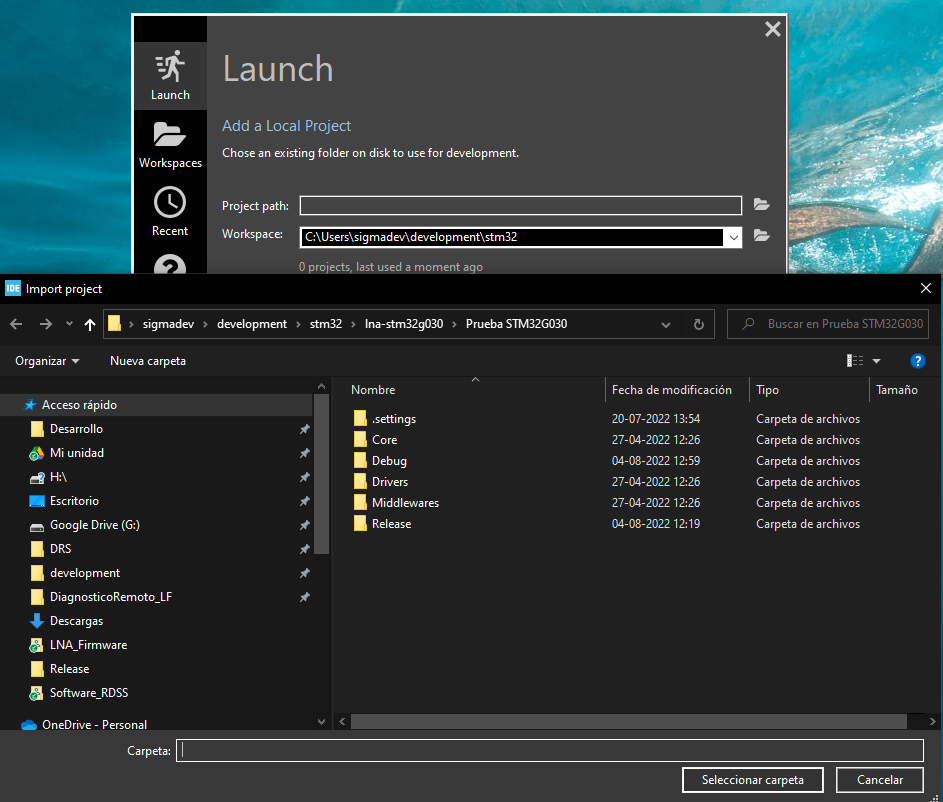
\includegraphics[width=0.8\textwidth]{figures/stm32cubeide1.png}
  \caption{Proyecto STM32}
    \label{fig:stm32-fylesystem}
\end{figure}

\newpage
\section{Descripción del Código}
Tras descargar el proyecto, examinamos el contenido de las carpetas /Core/Src y /Core/Inc. En la primera encontramos diversos archivos con extensión .c, mientras que en la segunda se ubican sus correspondientes archivos .h. Cabe destacar que aquellos archivos que comienzan con las palabras "stm32" y "sys" son generados automáticamente por el software y forman parte del controlador HAL. A continuación, se detallan los archivos que pertenecen a la capa de aplicación:

\begin{enumerate}
\setlength\itemsep{-0.1em}
\item eeprom: Este archivo contiene las funciones para leer y escribir en la memoria EEPROM.
\item utils: Este archivo contiene funciones para calcular el CRC16xModem~\cite{web:crc}.
\item main: Este archivo contiene el código para configurar las funciones del microcontrolador y las funciones para el correcto funcionamiento del LNA.
\end{enumerate}

Otro archivo importante es el LNA\_STM32G030.ioc, este archivo permite la configuración gráfica de los parámetros de operación del microcontrolador. Gráficamente se seleccionan las características y automáticamente se generan los códigos utilizando los controladores HAL. Este archivo se genera con la aplicación STM32CubeMx~\cite{web:stm32cubemx} que además crea el proyecto para comenzar a desarrollar. La figura \ref{fig:stm32cubemx} muestra el esquema del proyecto y como se ve el archivo de configuración LNA\_STM32G030.ioc:

\begin{figure}[H]
  \centering
   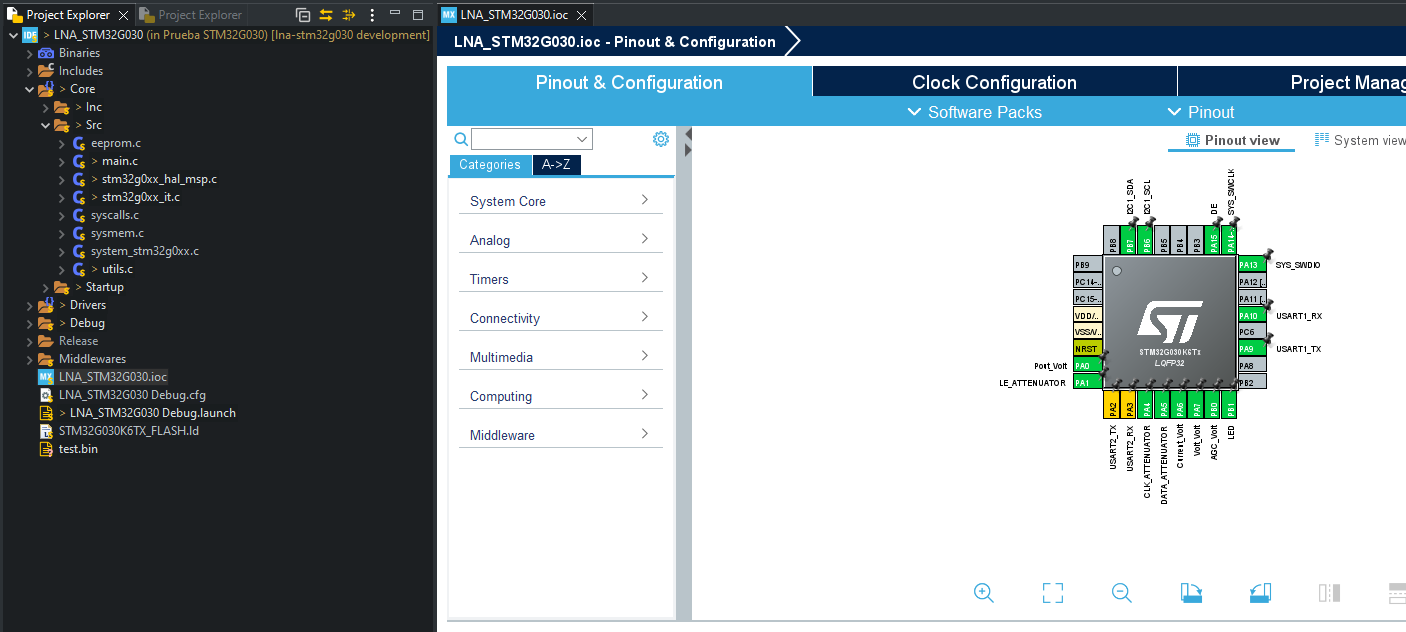
\includegraphics[width=0.9\textwidth]{figures/stm32cubemx.png}
  \caption{Esquema del proyecto}
    \label{fig:stm32cubemx}
\end{figure}

El esquema de la figura~\ref{fig:funciones} representa el diagrama de las funciones generales que realiza el firmware, estas son básicamente  tomar mediciones de los parámetros de operación a través del ADC, recibir comandos por la puerta serial y enviar información a través de la puerta serial.

\begin{figure}[H]
  \centering
   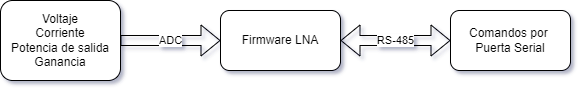
\includegraphics[width=0.9\textwidth]{figures/funciones.png}
  \caption{Esquema de funciones generales}
    \label{fig:funciones}
\end{figure}
\newpage
 A continuación se describen cada una de las funciones que componen la capa de aplicación y la figura~\ref{fig:codigo-esquema} muestra un esquema de flujo en el que se representa el sentido lógico de la ejecución del firmware. Es importante destacar que el nombre de las funciones es solo representativo para agrupar a un conjunto de acciones que se ejecutan en esa instancia.

\begin{figure}[H]
  \centering
   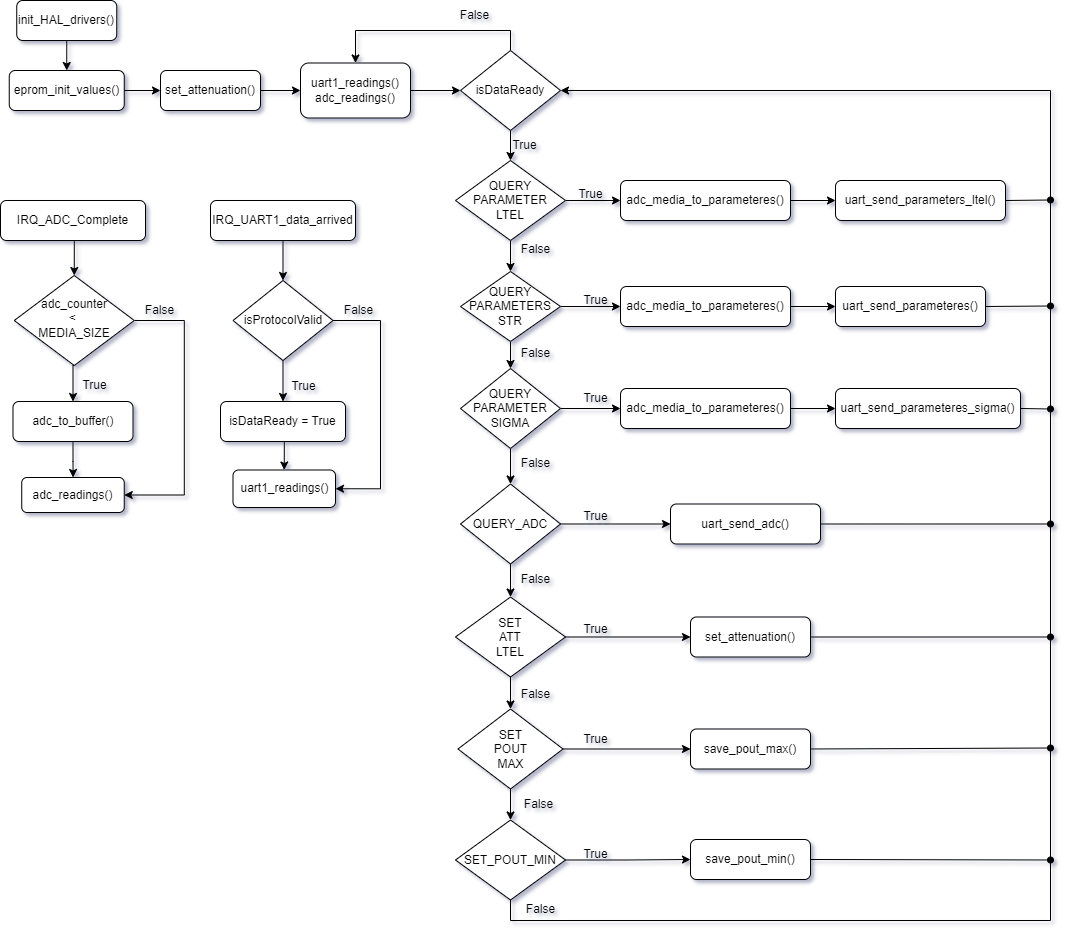
\includegraphics[width=\textwidth]{figures/diagrama_flujo.png}
  \caption{Diagrama conceptual}
    \label{fig:codigo-esquema}
\end{figure}

\begin{center}
\begin{tabular}{||r |m{10cm}| ||} 
 \hline
 \textbf{init\_HAL\_driver()} & Inicia los driver HAL para loss siguientes periféricos:
\begin{itemize}
\setlength\itemsep{-0.1em}
\item Acceso a la memoria del ADC y UART1 que no genera interrupciones en el código. 
\item Inicia qué pines serán de entrada y salida.
\item Inicia 4 canales del ADC para medir potencia de salida, consumo de corriente, ganancia y voltaje.
\item Inicia el driver i2C para la comunicación con la EEPROM.
\item Inicia el driver uart1 para la el envío y recepción de comandos.
\item Inicia el driver del Watchdog.
\end{itemize}
\\ \hline
\textbf{eeprom\_init\_values()} & Caga inicial de los parámetros de calibración en caso de estar calibrado, específicamente ajusta el valor máximo de la potencia de salida y el valor mínimo de la potencia de salida. \\ \hline 
\textbf{set\_attenuation()} & Se envía por UART1 la trama codificada que ajusta el valor de atenuación que está guardado en la EEPROM.\\ \hline 
\textbf{uart1\_readings()} & Espera por la lectura de 1 byte por la puerta serial uart1 y ejecuta una interrupción cuando llega algún dato. \\ \hline  
\textbf{adc\_readings()} & Ejecuta la lectura de los 4 canales del ADC y cuando termina se ejecuta una interrupción. \\ \hline
\textbf{IRQ\_ADC\_Complete} & Interrupción que se ejecuta cuando la conversión de los canales de los ADC está completa. \\ \hline
\textbf{adc\_to\_buffer()}  & Agrega cada lectura ADC a un buffer del tamaño MEDA\_SIZE. \\ \hline
\textbf{adc\_media\_to\_paramteres()} &  Calcula valor promedio parca de cada uno de los canales del ADC y con estos valores calcula los valores reales de potencia de salida, consumo de corriente, ganancia y voltaje. \\ \hline
\textbf{save\_pout\_max()} & Guarda el promedio actual del ADC de la potencia de salida como valor máximo. \\ \hline
\textbf{save\_pout\_min()} & Guarda el promedio actual del ADC de la potencia de salida como valor mínimo. \\ \hline
\textbf{uart\_send\_parameters\_letel()} & Codifica la trama según el protocolo de comunicación descrito en~\ref{sec:rs485}para ser compatible por el software \textbf{BDA TEST SOFT} del proveedor LTEL y los envía por la puerta serial uart1, más detalles de los parametros en~\ref{sec:ltel-param}. \\ \hline
\textbf{uart\_send\_parameters\_sigma()} & Codifica la trama según el protocolo de comunicación descrito en~\ref{sec:rs485} agregando los nuevos valores de SIGMA y los envía por la puerta serial uart1, más detalles de los parámetros en~\ref{sec:sigma-param}. \\ \hline
\textbf{uart\_send\_parameters()} & Entrega los valores promedios de los parámetros en modo texto para revisión técnica,  más detalles de los parámetros~\ref{sec:str-param}. \\ \hline
\textbf{uart\_send\_adc()} & Entrega los valores medios de los 4 canales del ADC,  más detalles de los parámetros~\ref{sec:adc-param}. \\ \hline
\end{tabular}
\end{center}


%\begin{itemize}
%\setlength\itemsep{-0.1em}
%\item Acceso a la memoria del ADC y UART1 que no genera interrupciones en el código. 
%\item Inicia qué pines serán de entrada y salida.
%\item Inicia 4 canales del ADC para medir potencia de salida, consumo de corriente, ganancia y voltaje.
%\item Inicia el driver i2C para la comunicación con la EEPROM.
%\item Inicia el driver uart1 para la el envío y recepción de comandos.
%\item Inicia el driver del Watchdog.
%\end{itemize}

%\paragraph{eeprom\_init\_values()} Caga inicial de los parámetros de calibración en caso de estar calibrado, específicamente ajusta el valor máximo de la potencia de salida y el valor mínimo de la potencia de salida. 
%\paragraph{set\_attenuation()} Se envía por UART1 la trama codificada que ajusta el valor de atenuación que 
%\paragraph{uart1\_readings()} Espera por la lectura de 1 byte por la puerta serial uart1 y ejecuta una interrupción cuando llega algún dato.
%\paragraph{adc\_readings()} Ejecuta la lectura de los 4 canales del ADC y cuando termina se ejecuta una interrupción.
%\paragraph{IRQ\_ADC\_Complete} Interrupción que se ejecuta cuando la conversión de los canales de los ADC está completa.
%\paragraph{adc\_to\_buffer()}  Agrega cada lectura ADC a un buffer del tamaño MEDA\_SIZE.
%\paragraph{adc\_media\_to\_paramteres()} Función que calcula valor promedio con MEDIA\_SIZE muestrada parca de cada uno de los canales del ADC y con los valores promedio calcula la potencia de salida, consumo de corriente, ganancia y voltaje.
%\paragraph{save\_pout\_max()} Guarda el promedio actual del ADC de la potencia de salida como valor máximo.
%\paragraph{save\_pout\_min()} Guarda el promedio actual del ADC de la potencia de salida como valor mínimo.
%\paragraph{uart\_send\_parameters\_letel()} Codifica la trama según el protocolo de comunicación descrito en~\ref{sec:rs485}para ser compatible por el software \textbf{BDA TEST SOFT} del proveedor LTEL y los envía por la puerta serial uart1, más detalles de los parametros en~\ref{sec:ltel-param}.
%\paragraph{uart\_send\_parameters\_sigma()} Codifica la trama según el protocolo de comunicación descrito en~\ref{sec:rs485} agregando los nuevos valores de SIGMA y los envía por la puerta serial uart1, más detalles de los parámetros en~\ref{sec:sigma-param}.
%\paragraph{uart\_send\_parameters()} Entrega los valores promedios de los parámetros en modo texto para revisión técnica,  más detalles de los parámetros~\ref{sec:str-param}.
%\paragraph{uart\_send\_adc()} Entrega los valores medios de los 4 canales del ADC,  más detalles de los parámetros~\ref{sec:adc-param}.

\section{Carga de firmware desde ST32CubeIDE}
Conectar el depurador al LNA con el Pinout indicado en la figura~\ref{fig:lna_completo} y cargar el proyecto al software ST32CubeIDE~\ref{sec:repo}. Si el depurador es reconocido simplemte ejectuar \textbf{RUN} como se muestra en la figura~\ref{fig:stm32-run}

\begin{figure}[H]
  \centering
   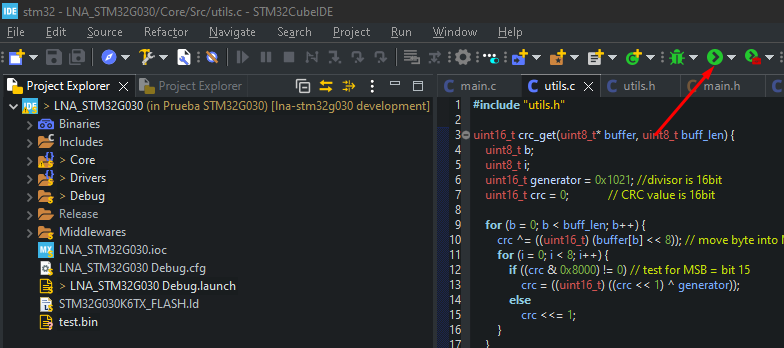
\includegraphics[width=0.8\textwidth]{figures/stm32-run.png}
  \caption{Cargar firmware con STM32CubeIDE}
    \label{fig:stm32-run}
\end{figure}

En caso de éxito el mensaje en la figura~\ref{fig:stm32-run-ok} en la pestañana Consola debería aparecer, de lo contrario revisar los pasos anteriores.

\section{Carga de firmware STM32CubeProgrammer}
Conectar el depurador al LNA con el Pinout indicado en la figura~\ref{fig:lna_completo}.
\begin{enumerate}
\setlength\itemsep{-0.1em}
    \item Conectar el depurador con el software.
    \item Buscar el archivo .elf.
\end{enumerate}

\begin{figure}[H]
  \centering
   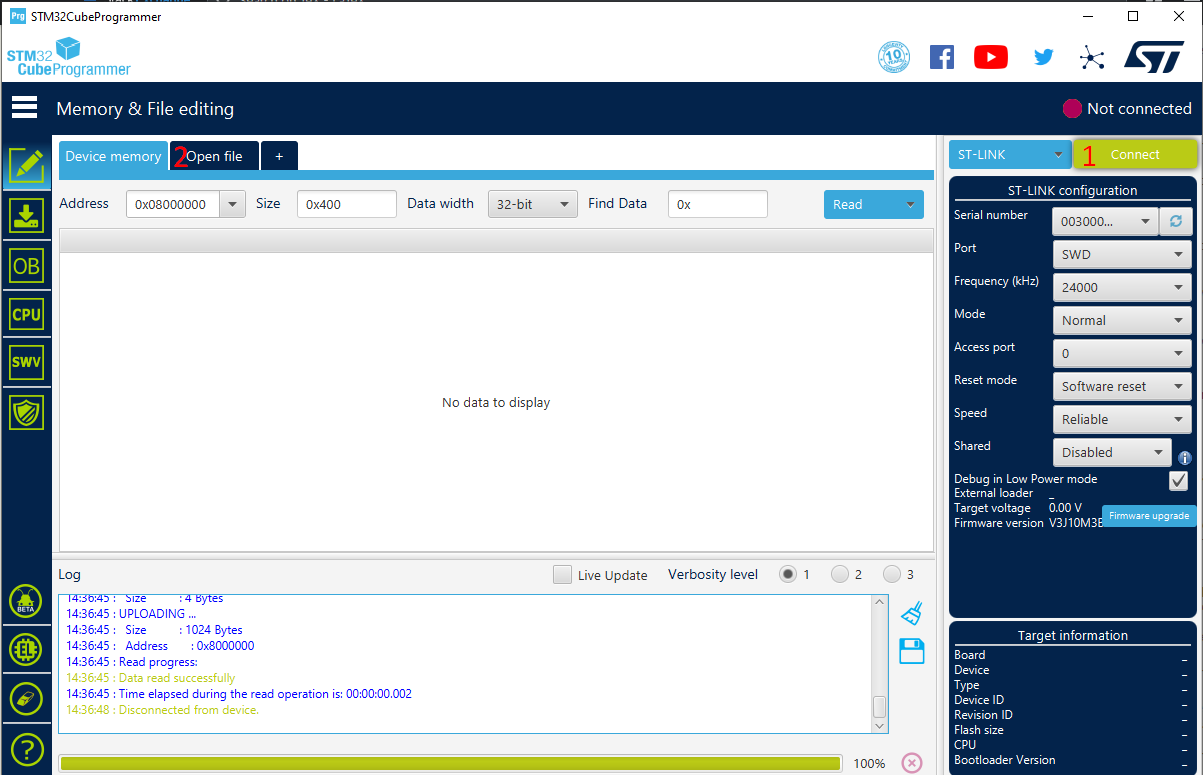
\includegraphics[width=0.7\textwidth]{figures/programmer.png}
  \caption{Cargar firmware con STM32CubeProgrammer}
    \label{fig:stm32-run-ok}
\end{figure}

Una vez conseguir el archivo .elf, en este ejemplo como LNA\_STM32G030.elf, seleccionar Download y listo. En caso de éxito el mensaje en la figura~\ref{fig:stm32-run-ok}, de lo contrario revisar los pasos anteriores.

\begin{figure}[H]
  \centering
   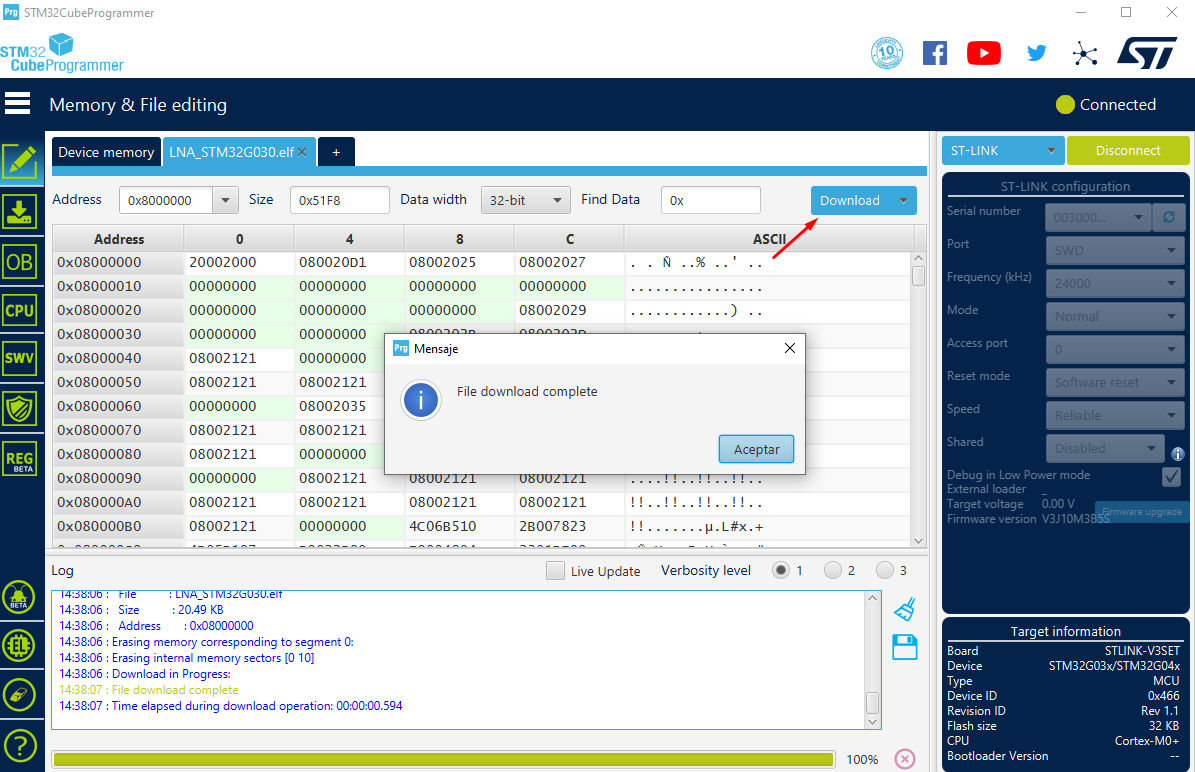
\includegraphics[width=0.7\textwidth]{figures/programmer_download.png}
  \caption{Cargar firmware con STM32CubeProgrammer}
    \label{fig:stm32-run-ok}
\end{figure}

\newpage
\section{Protocolo de Comunicación por RS-485}\label{sec:rs485}
La placa tiene un puerto de comunicación RS-485 y un protocolo de comunicación que consiste en enviar una trama que tiene la siguiente estructura.
\begin{center}
\begin{tabular}{||c | l | l||} 
 \hline
 bytes & Nombre & Valor Hex para el LNA \\ [0.5ex] 
 \hline\hline
 1 [MSB] &  Inicio de trama & 0x7E para todos\\ 
 \hline
 1 &  Función del módulo & 0x09 para LNA \\
 \hline
 1 &  Dirección del módulo & Es un identificador en caso de usar más de un LNA \\ 
 \hline
 n &  Comando  & Depende del comando \\
 \hline
 2 &  CRC  & Se calcula según CRC-16/XMODEM~\cite{web:crc} \\
 \hline
 1 [LSB]&  Fin de trama & 0x7F para todos \\
 \hline
 \hline
\end{tabular}
\end{center}

\section{Calibración}
Debido a la naturaleza del detector LMV221~\cite{web:lmv221} de la potencia de salida, se debe realizar una calibración para cada placa al momento de las pruebas, el rango dinámico del detector es de 30[dBm]. Para realizar la calibración se generan comandos que se envían a través de la comunicación RS-485. El procedimiento para calibrar es: 
\begin{enumerate}
\setlength\itemsep{-0.1em}
    \item Medir potencia de salida con un analizador.
    \item Inyectar potencia hasta que la salida llegue a su máximo valor, alrededor de 0 [dBm].
    \item Enviar el comando de guardar potencia máxima.
    \item Inyectar potencia hasta que el valor de salida llegue a -30 [dBm].
    \item Enviar el comando de guardar potencia mínima. 
\end{enumerate}
Con estos pasos la medición del LNA quedará calibrada para el rango de -30[dBm] a 0[dBm].

\section{Comandos}

Para el envío de comandos se utiliza la misma estructura de trama de LTEL, el proveedor inicial. Además se incluyen otros comandos con funcionalidades extras.Para una explicación más clara se muestra solo el valor HEX del comando pero hay que recordar que se debe enviar la trama completa descrita en la sección~\ref{sec:rs485}. 

\subsection{Ajuste de atenuación - 0x200000}
La atenuación se puede ajustar desde 0 [dB] hasta 31 [dB], para esto se envía la trama 0x2000\textbf{00} en donde el último byte corresponde al valor de la atenuación en hexadecimal. Por ejemplo, para ajustar la atenuación a 20[dB] se envía la siguiente trama.
\begin{minted}[bgcolor=black]{r}
\$ Query: 20000014
\$ Answer:
\end{minted}
 El comando no tiene respuesta.

\subsection{Ajuste de Potencia Máxima de calibración - 0x240000}
Guarda el valor máximo actual del promedio del ADC de la potencia de salida. Este valor sirve para calibrar la potencia de salida. Un ejemplo sería.
\begin{minted}[bgcolor=black]{r}
\$ Query: 240000
\$ Answer: "Saved Pout max value"
\end{minted}

\subsection{Ajuste de Potencia Mínima de calibración - 0x230000}
Guarda el valor mínimo actual del promedio del ADC de la potencia de salida. Este valor sirve para calibrar la potencia de salida. Un ejemplo sería.
\begin{minted}[bgcolor=black]{r}
\$ Query: 230000
\$ Answer: "Saved Pout max value"
\end{minted}

\subsection{Consulta de parámetros - 0x110000}\label{sec:ltel-param}
Para la consulta de parámetros del software de LTEL y mantener la compatibilidad, se envía la trama 0x110000. Un ejemplo sería:
\begin{minted}[bgcolor=black]{r}
\$ Query: 110000
\$ Answer: 110005000a2ce8e8
\$ Decode: Gain:44[dBm] ATT:10[dB] OutputPower:-24[dBm] InputPower:-24[dBm]
\end{minted}

La respuesta es un número hexadecimal que tiene la siguiente estructura:
\begin{itemize}
\setlength\itemsep{-0.1em}
    \item (uint8\_t) 0x11: id del comando
    \item (uint8\_t) 0x05: número de parámetros de 1 byte.
    \item (uint8\_t) 0x00: indefinido
    \item (uint8\_t) 0x0a: atenuación
    \item (uint8\_t) 0x2c: ganancia
    \item \textbf{(sint8\_t)} 0xe8: potencia de salida 
    \item (uint8\_t) 0xe8: indefinido
\end{itemize}

El valor Decode sería la trama decodificada según el número hexadecimal recibido.

\subsection{Consulta de parámetros - Sigma - 0x120000}\label{sec:sigma-param}
Para la consulta de parámetros sigma, se envía la trama 0x120000. Ejemplo:
\begin{minted}[bgcolor=black]{r}
\$ Query: 120000
\$ Answer: 1206e2002d660eb5
\$ Decode: "OutputPower:-30dBm] ATT:0[dB] Gain: 45[dB] InputPower:-75[dBm]
Current: 102[mA] Voltage: 14[v]" 
\end{minted}

La respuesta es un número hexadecimal que tiene la siguiente estructura:
\begin{itemize}
\setlength\itemsep{-0.1em}
    \item (uint8\_t) 0x12: id del comando
    \item (uint8\_t) 0x06: número de parámetros de 1 byte
    \item \textbf{(sint8\_t)} 0xe2: potencia de salida en [dBm] 
    \item (uint8\_t) 0x00: atenuación en [dB]
    \item (uint8\_t) 0x2d: ganancia en [dB]
    \item (uint8\_t) 0x66: corriente de consumo en [mA]
    \item \textbf{(uint8\_t)} 0x0e: voltaje de entrada en [V]
    \item (sint8\_t) 0xb5: potencia de entrada calculada en [dBm]
\end{itemize}

El valor Decode sería la trama decodificada según el número hexadecimal recibido.

\subsection{Lecturas decodificadas - 0x150000}\label{sec:str-param}
Un comando extra para uso técnico. Se puede consultar los parámetros y los entrega decodificados. Para esto enviar 150000. Un ejemplo de la consulta.

\begin{minted}[bgcolor=black]{r}
\$ Query: 150000
\$ Answer:"Pout -31[dBm] ATT 0[dB] Gain 44[dB] Pin -75[dBm] Curent 96[mA]
Voltage 14[V]"
\end{minted}

\subsection{Valores ADC - 0x160000}\label{sec:adc-param}
Un comando extra para uso técnico. Se puede consultar los valores ADC promedio actuales en caso de codificarlos de manera centralizada. Para esto enviar 160000. Un ejemplo de la consulta
\begin{minted}[bgcolor=black]{r}
\$ Query: 160000
\$ Answer:"Pout 1234 Att 231  Gain 255  Curent 1002 Voltage 462"
\end{minted}

\subsection{Lista de comandos}
A continuación un resumen de los comandos para un LNA 0x09 con ID 0x08. Estas consultas sirven para realizar consultas rápidas de forma manual con un programa que pueda enviar datos por la puerta serial como Hercules~\cite{web:hercules}
\begin{center}
\begin{tabular}{||c | l c c||} 
 \hline
 N & Comando & Comando hex & Trama completa \\ [0.5ex] 
 \hline\hline
 1 & Guarda el ADC promedio de potencia máxima & 240000 & 7e0908240000b9777f \\ 
 \hline
 3 & Guarda el ADC promedio de potencia mínima & 230000 & 7e090823000029f27f \\ 
 \hline
 5 & Cambiar atenuación a 16[dB]& 20000010 & 7e090820000010b06f7f \\
 \hline
  6 & Consulta de parámetros LTEL & 110000 & 7e0908110000ec597f \\
  \hline
  7 & Consultar de parámetros Sigma & 120000 &  7e0908120000bc7f \\
 \hline
 8 & Consultar parámetros en modo Texto & 150000 &  7e09081500002c857f \\
 \hline
  8 & Consultar valores ADC & 160000 &  7e09081600007cdc7f \\
 \hline
 
\end{tabular}
\end{center}


\section{Versiones del Firmware}
La tabla describe la versión, la fecha y las características principales.
\begin{center}
\begin{tabular}{||c | c | |m{10cm}| ||} 
 \hline
Versión & Fecha & Cambios \\ [0.5ex] 
\hline

 2 & 02/08/2022 & \begin{itemize}
 \setlength\itemsep{-0.1em}
\item Ajuste de atenuación por RS-485
\item Lectura de Voltaje (solo para los UHF).
\item Lectura de ADC promediada.
\item Lectura de protocolo RS-485 simplificada.
\item Comando para consultar todos los parámetros.
 \end{itemize}
 \\ 
 \hline
 1 & 21/07/2022 & \begin{itemize}
 \setlength\itemsep{-0.1em}
     \item Compatibilidad con el software BDA
\item Ajuste de atenuación por RS-485
\item Lectura de Ganancia.
\item Lectura de Potencia de salida
\item Lectura de consumo de corriente
\item Calculo de Potencia de entrada
\item Calibración para el sensor de Pout por RS-485
 \end{itemize}
 \\ 
\hline

\end{tabular}
\end{center}
%\begin{figure}
%  \centering
%   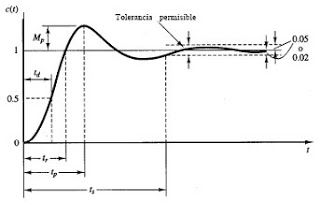
\includegraphics[width=0.7\textwidth]{figures/2orden}
%  \caption{Especificaciones de la respuesta transitoria}
%  \label{fig:2orden}
%\end{figure}
%%
\newpage

\section{Revisión del documento}

\begin{center}
\begin{tabular}{||c | c |c | |m{5cm}||} 
 \hline
Autor & Correo & Fecha & Cambios \\ [0.5ex] 
\hline
 \hline
 Arturo Veras &arturo@sigma-telecom.com &  22/08/2022 & 
 \begin{itemize}
 \setlength\itemsep{-0.1em}
      \item Inicio del coumento.
 \end{itemize}
 \\ 
\hline

\end{tabular}
\end{center}

\newpage
\bibliographystyle{plain}

\bibliography{Bibliography}{}


\end{document}
